% Paper-style visual architecture: real input/output, stacked feature maps,
% functional regions, and an expanded geometry-aware block.
\newcommand{\featurestack}[7]{%
  \begin{scope}[shift={(#2,#3)}]
    \foreach \k in {3,2,1,0}{
      \draw[draw=#4!75!black, fill=#4!22, line width=0.4pt]
        ({-#5/2+0.07*\k},{-#6/2+0.07*\k}) rectangle
        ({#5/2+0.07*\k},{#6/2+0.07*\k});
    }
  \end{scope}
  \node[minimum width=#5cm, minimum height=#6cm, inner sep=0pt] (#1) at (#2,#3) {};
  \node[font=\sffamily\footnotesize, align=center, anchor=north] at ($(#1.south)+(0,-0.10)$) {#7};
}

\begin{tikzpicture}[
  font=\sffamily\footnotesize,
  >=Latex,
  flow/.style={->, very thick, draw=black!75},
  thinflow/.style={->, thick, draw=black!65},
  featureflow/.style={->, thick, draw=blue!65!black},
  residual/.style={->, thick, dashed, draw=orange!85!black},
  unit/.style={draw=black!70, rounded corners=2pt, align=center, minimum height=8mm,
      fill=white, inner sep=2.3pt},
  encoder/.style={unit, fill=cyan!15, draw=cyan!60!black, minimum width=25mm},
  down/.style={unit, fill=gray!12, draw=gray!60, minimum width=21mm},
  msa/.style={unit, fill=blue!10, draw=blue!65!black},
  deg/.style={unit, fill=red!9, draw=red!60!black},
  ocv/.style={unit, fill=green!11, draw=green!55!black},
  gbc/.style={unit, fill=orange!13, draw=orange!75!black},
  srf/.style={unit, fill=blue!7, draw=blue!45!black},
  head/.style={unit, fill=orange!20, draw=orange!75!black, minimum width=10mm,
      minimum height=18mm},
  gate/.style={draw=black!75, circle, fill=yellow!18, minimum size=5.5mm,
      inner sep=0.4pt, font=\sffamily\scriptsize\bfseries},
  op/.style={draw=black!65, circle, fill=white, minimum size=5.5mm,
      inner sep=0.3pt, font=\scriptsize\bfseries},
  mini/.style={draw=black!60, rounded corners=1pt, align=center,
      fill=white, inner sep=1.5pt, font=\sffamily\scriptsize},
  title/.style={font=\sffamily\small\bfseries, anchor=west}
]

% ==================================================================
% (a) Overall architecture
% ==================================================================
\filldraw[rounded corners=3pt, fill=gray!2, draw=gray!18] (0,6.25) rectangle (19.5,12.0);
\node[title] at (0.25,11.72) {(a) Overall architecture of MSA--OCV--GBC MixerCSeg};

\node[draw=black!55, inner sep=1pt] (imgin) at (0.85,8.95)
  {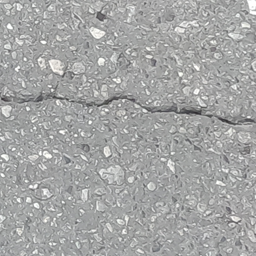
\includegraphics[width=1.45cm]{../dataset/CrackMap/test_img/GOPR0317 (5).png}};
\node[font=\scriptsize, below=0.8mm of imgin] {Input};
\node[unit, fill=orange!12, minimum width=9mm, minimum height=22mm] (stem) at (2.35,8.95)
  {Stem};
\draw[flow] (imgin) -- (stem);

% Encoder with stage hierarchy and 3-D multi-scale outputs.
\filldraw[rounded corners=3pt, fill=cyan!4, draw=cyan!25] (3.00,6.62) rectangle (7.35,11.38);
\draw[dashed, thick, draw=black!50, rounded corners=2pt] (3.25,6.88) rectangle (5.80,11.10);
\node[font=\scriptsize\bfseries] at (4.53,10.88) {Four-stage encoder};
\node[encoder] (e1) at (4.53,10.22) {TransMixer + GAB\\$16\!\times128^2$};
\node[down] (pm) at (4.53,9.26) {Patch Merging $\downarrow2$};
\node[font=\Large] at (4.53,8.56) {$\vdots$};
\node[encoder] (e4) at (4.53,7.65) {TransMixer + GAB\\$128\!\times16^2$};
\draw[thinflow] (e1) -- (pm);
\draw[thinflow] (pm) -- (e4);
\draw[flow] (stem) -- (e1.west);

\featurestack{f1}{6.46}{10.38}{cyan}{0.72}{0.80}{$F_1$}
\featurestack{f2}{6.66}{9.48}{blue}{0.62}{0.69}{$F_2$}
\featurestack{f3}{6.85}{8.60}{blue}{0.53}{0.59}{$F_3$}
\featurestack{f4}{7.02}{7.75}{blue}{0.44}{0.49}{$F_4$}
\draw[featureflow] (e1.east) -- (f1.west);
\draw[featureflow] (5.58,9.50) -- (f2.west);
\draw[featureflow] (5.58,8.62) -- (f3.west);
\draw[featureflow] (e4.east) -- (f4.west);

% SRF decoder mirrors the implemented attention and fusion path.
\filldraw[rounded corners=3pt, fill=blue!4, draw=blue!22] (7.55,6.62) rectangle (16.15,11.38);
\node[font=\small\bfseries, anchor=west] at (7.80,11.10) {SRF decoder};
\node[srf, minimum width=18mm] (p1) at (8.55,10.10) {$F_1$ projection\\$16\!\rightarrow8$};
\node[srf, minimum width=18mm] (p234) at (8.55,7.75) {$F_{2:4}$ projection\\$\{32,64,128\}\!\rightarrow8$};
\node[srf, minimum width=16mm] (att) at (10.72,10.10) {$1{\times}1$ Conv\\$A=\sigma(\cdot)$};
\node[srf, minimum width=15mm] (up1) at (12.65,10.10) {Upsample\\to $512^2$};
\node[srf, minimum width=18mm] (align) at (11.02,7.75) {Upsample $F_{2:4}$\\to $128^2$};
\node[op] (mul) at (12.38,7.75) {$\odot$};
\node[srf, minimum width=15mm] (up234) at (13.48,7.75) {Upsample\\to $512^2$};
\node[srf, minimum width=10mm, minimum height=14mm] (cat) at (14.52,9.05) {Cat\\32 ch};
\node[srf, minimum width=10mm, minimum height=14mm] (fuse) at (15.48,9.05) {Fuse\\8 ch};

\draw[featureflow] (f1.east) -- (p1.west);
\draw[featureflow] (f2.east) -| (p234.north west);
\draw[featureflow] (f3.east) -- (p234.west);
\draw[featureflow] (f4.east) -| (p234.south west);
\draw[flow] (p1) -- (att);
\draw[flow] (att) -- (up1);
\draw[flow] (p234) -- (align);
\draw[flow] (align) -- (mul);
\draw[flow] (att.south) |- (mul.north);
\draw[flow] (mul) -- (up234);
\draw[flow] (up1.east) -| (cat.north);
\draw[flow] (up234.east) -| (cat.south);
\draw[flow] (cat) -- (fuse);

\node[head] (seg) at (16.85,9.05) {Seg\\Head};
\node[draw=black!55, inner sep=1pt] (imgout) at (18.55,9.05)
  {\includegraphics[width=1.45cm]{../results/probability_maps/triple_stack_v4_crackmap/validate_v3_msa_ocv_gbc_seed42/GOPR0317 (5)_pre.png}};
\node[font=\scriptsize, below=0.8mm of imgout] {Output};
\draw[flow] (fuse) -- (seg);
\draw[flow] (seg) -- (imgout);

% ==================================================================
% (b) Expanded GAB, with simplified icons for visual readability.
% Exact equations remain in Figure 3 and the method text.
% ==================================================================
\filldraw[rounded corners=3pt, fill=gray!1, draw=black!45, line width=0.7pt]
  (0,0) rectangle (19.5,5.90);
\node[title] at (0.25,5.60) {(b) Geometry-aware block (GAB) after each TransMixer};

\featurestack{xin}{0.62}{3.00}{cyan}{0.55}{1.20}{$\mathbf{X}$}

% MSA.
\filldraw[rounded corners=2pt, fill=blue!3, draw=blue!35] (1.25,0.82) rectangle (4.65,5.05);
\node[font=\small\bfseries, text=blue!65!black] at (2.95,4.78) {MSA};
\node[msa, minimum width=10mm] (mh) at (2.00,4.00) {$1{\times}9$};
\node[msa, minimum width=10mm] (mv) at (2.00,3.20) {$9{\times}1$};
\node[msa, minimum width=10mm] (md) at (2.00,2.40) {Dilated};
\node[msa, minimum width=11mm] (mrc) at (2.00,1.55) {Row/col};
\node[msa, minimum width=15mm, minimum height=18mm] (mf) at (3.65,2.85) {Concat\\$1{\times}1$\\GN};
\draw[thinflow] (xin.east) -- (mh.west);
\draw[thinflow] (xin.east) -- (mv.west);
\draw[thinflow] (xin.east) -- (md.west);
\draw[thinflow] (xin.east) |- (mrc.west);
\draw[thinflow] (mh.east) -- (mf.west);
\draw[thinflow] (mv.east) -- (mf.west);
\draw[thinflow] (md.east) -- (mf.west);
\draw[thinflow] (mrc.east) -- (mf.south west);
\featurestack{xm}{4.95}{3.00}{blue}{0.44}{1.00}{MSA}
\node[gate] (g1) at (5.55,3.00) {$\mathcal{G}_1$};

% Inherited DEGConv.
\node[deg, minimum width=12mm, minimum height=16mm] (deg) at (6.35,3.00) {DEG\\Conv};
\draw[flow] (mf.east) -- (xm.west);
\draw[flow] (xm) -- (g1);
\draw[flow] (g1) -- (deg);

% OCV.
\filldraw[rounded corners=2pt, fill=green!3, draw=green!35] (6.95,0.82) rectangle (11.00,5.05);
\node[font=\small\bfseries, text=green!50!black] at (8.98,4.78) {OCV};
\node[ocv, minimum width=11mm] (os) at (7.70,4.00) {Sobel};
\node[ocv, minimum width=11mm] (oh) at (7.70,3.05) {Hessian};
\node[ocv, minimum width=11mm] (oa) at (7.70,2.10) {Axial};
\node[ocv, minimum width=13mm, minimum height=15mm] (vote) at (9.05,3.05) {Vote\\$Q$};
\node[ocv, minimum width=13mm, minimum height=18mm] (of) at (10.25,3.05) {Concat\\$1{\times}1$\\GN};
\draw[thinflow] (deg.east) -- (os.west);
\draw[thinflow] (deg.east) -- (oh.west);
\draw[thinflow] (deg.east) -- (oa.west);
\draw[thinflow] (os.east) -- (vote.west);
\draw[thinflow] (oh.east) -- (vote.west);
\draw[thinflow] (oa.east) -- (vote.west);
\draw[thinflow] (vote) -- (of);
\featurestack{xo}{11.28}{3.00}{green}{0.44}{1.00}{OCV}
\node[gate] (g2) at (11.88,3.00) {$\mathcal{G}_2$};

% GBC.
\filldraw[rounded corners=2pt, fill=orange!4, draw=orange!45] (12.25,0.82) rectangle (16.55,5.05);
\node[font=\small\bfseries, text=orange!75!black] at (14.40,4.78) {GBC};
\node[gbc, minimum width=12mm] (gap) at (13.05,4.00) {Gap};
\node[gbc, minimum width=12mm] (bound) at (13.05,3.05) {Boundary};
\node[gbc, minimum width=12mm] (entropy) at (13.05,2.10) {Entropy};
\node[gbc, minimum width=14mm] (conf) at (14.45,3.55) {Confidence\\$C_g$};
\node[gbc, minimum width=14mm] (bridge) at (14.45,2.30) {Bridge\\$Z$};
\node[gbc, minimum width=13mm, minimum height=18mm] (gf) at (15.78,3.05) {Concat\\$1{\times}1$\\GN};
\draw[thinflow] (g2.east) -- (gap.west);
\draw[thinflow] (g2.east) -- (bound.west);
\draw[thinflow] (g2.east) -- (entropy.west);
\draw[thinflow] (gap.east) -- (conf.west);
\draw[thinflow] (bound.east) -- (conf.west);
\draw[thinflow] (entropy.east) -- (bridge.west);
\draw[thinflow] (conf) -- (bridge);
\draw[thinflow] (bridge) -- (gf);

\node[gate] (g3) at (16.90,3.00) {$\mathcal{G}_3$};
\node[unit, fill=gray!10, minimum width=8mm] (gn) at (17.60,3.00) {GN};
\featurestack{yout}{18.60}{3.00}{purple}{0.55}{1.20}{$\mathbf{Y}$}
\draw[flow] (gf) -- (g3);
\draw[flow] (g3) -- (gn);
\draw[flow] (gn) -- (yout.west);

\draw[residual] (xin.south) -- ++(0,-1.85) -| (yout.south);
\node[font=\scriptsize, fill=white, inner sep=1pt] at (9.75,0.55)
  {stage-level residual gate $\mathcal{G}_{f}$};
\node[font=\scriptsize, text=gray!70!black, anchor=west] at (0.35,0.25)
  {Stacked planes represent feature tensors; full branch equations and channel concatenations are expanded in Fig.~3.};

\end{tikzpicture}
